% \documentclass[aspectratio=169,notes]{beamer}
\documentclass[aspectratio=169]{beamer}
\usetheme[faculty=phil]{fibeamer}
\usepackage{polyglossia}
\setmainlanguage{english} %% main locale instead of $english$, you
%% can typeset the presentation in either Czech or Slovak,
%% respectively.
\setotherlanguages{russian} %% The additional keys allow
%%
%%   \begin{otherlanguage}{czech}   ... \end{otherlanguage}
%%   \begin{otherlanguage}{slovak}  ... \end{otherlanguage}
%%
%% These macros specify information about the presentation
\title[Artificial Intelligence Software (AIS)]{Artificial Intelligence Software, Lab 3} %% that will be typeset on the
\subtitle{ROS 2:  
\\ Simulators, TF2, URDF, DDS, Tests \\ \  } %% title page.
\author{Oleg Bulichev}
%% These additional packages are used within the document:
\usepackage{ragged2e}  % \justifying text
\usepackage{dirtree}
\usepackage{booktabs}  % Tables
\usepackage{tabularx}
\usepackage{tikz}      % Diagrams
\usetikzlibrary{calc, shapes, backgrounds, arrows.meta, positioning}
\usetikzlibrary{decorations.pathreplacing,calligraphy,calc,graphs}
\usepackage{amsmath, amssymb}
\usepackage{url}       % \urls
\usepackage{listings}  % Code listings
% \usepackage{subfigure}
\usepackage{floatrow}
\usepackage{subcaption}
\usepackage{mathtools}
\usepackage{todonotes}
\usepackage{fontspec}
\usepackage{multicol}
\usepackage{pdfpages}
\usepackage{wrapfig}
\usepackage{qrcode}
\usepackage{animate}
\usepackage{booktabs}
\usepackage{multirow}
% \usepackage{graphicx}
\usepackage{colortbl}

\graphicspath{{resources/}}
\frenchspacing

\setbeamertemplate{caption*}[numbered]
\usetikzlibrary{graphs}

\newcommand{\oleg}[2][] {\todo[color=red, #1] {OLEG:\\ #2}}
\newcommand{\fbckg}[1]{\usebackgroundtemplate{\includegraphics[width=\paperwidth]{#1}}}%frame background

\usepackage[framemethod=TikZ]{mdframed}
\newcommand{\dbox}[1]{
\begin{mdframed}[roundcorner=3pt, backgroundcolor=yellow, linewidth=0]
\vspace{1mm}
{#1}
\vspace{1mm}
\end{mdframed}
}

\lstset{
  basicstyle=\ttfamily\tiny,
  keywordstyle=\color{blue},
  stringstyle=\color{red},
  commentstyle=\color{green!50!black},
  morecomment=[l][\color{magenta}]{\#},
  frame=single,
  breaklines=true,
  showstringspaces=false
}

\begin{document}
\setlength{\abovedisplayskip}{0pt}
\setlength{\belowdisplayskip}{0pt}
\setlength{\abovedisplayshortskip}{0pt}
\setlength{\belowdisplayshortskip}{0pt}

\fbckg{fibeamer/figs/title_page.png}
\frame[c]{\setcounter{framenumber}{0}
    \usebeamerfont{title}%
    \usebeamercolor[fg]{title}%
    \begin{minipage}[b][6.5\baselineskip][b]{\textwidth}%
        \textcolor{black}{\raggedright\inserttitle}
    \end{minipage}
    % \vskip-1.5\baselineskip

    \usebeamerfont{subtitle}%
    \usebeamercolor[fg]{framesubtitle}%
    \begin{minipage}[b][3\baselineskip][b]{\textwidth}
        \raggedright%
        \insertsubtitle%
    \end{minipage}
    \vskip.25\baselineskip
}

\fbckg{fibeamer/figs/common.png}

% --- CHAPTER 1: SIMULATORS ---
\section{Physics Engines \& Simulators}

\begin{frame}[t]{Introduction to Simulators}
    \begin{columns}
        \column{0.6\textwidth}
        \begin{itemize}
            \item \textbf{What is a Simulator?} A software environment that mimics the physical world, allowing robots to be tested virtually.
            \item \textbf{Why use them?}
            \begin{itemize}
                \item \textbf{Safety:} No risk of breaking expensive hardware.
                \item \textbf{Speed:} Can run faster than real-time.
                \item \textbf{Cost:} Free to create complex scenarios.
            \end{itemize}
            \item \textbf{Key Components:}
            \begin{itemize}
                \item \textbf{Rendering Engine:} Visual output.
                \item \textbf{Physics Engine:} Dynamics \& Collisions.
                \item \textbf{ROS Interface:} Bridge to ROS 2.
            \end{itemize}
        \end{itemize}
        \column{0.4\textwidth}
        \centering
        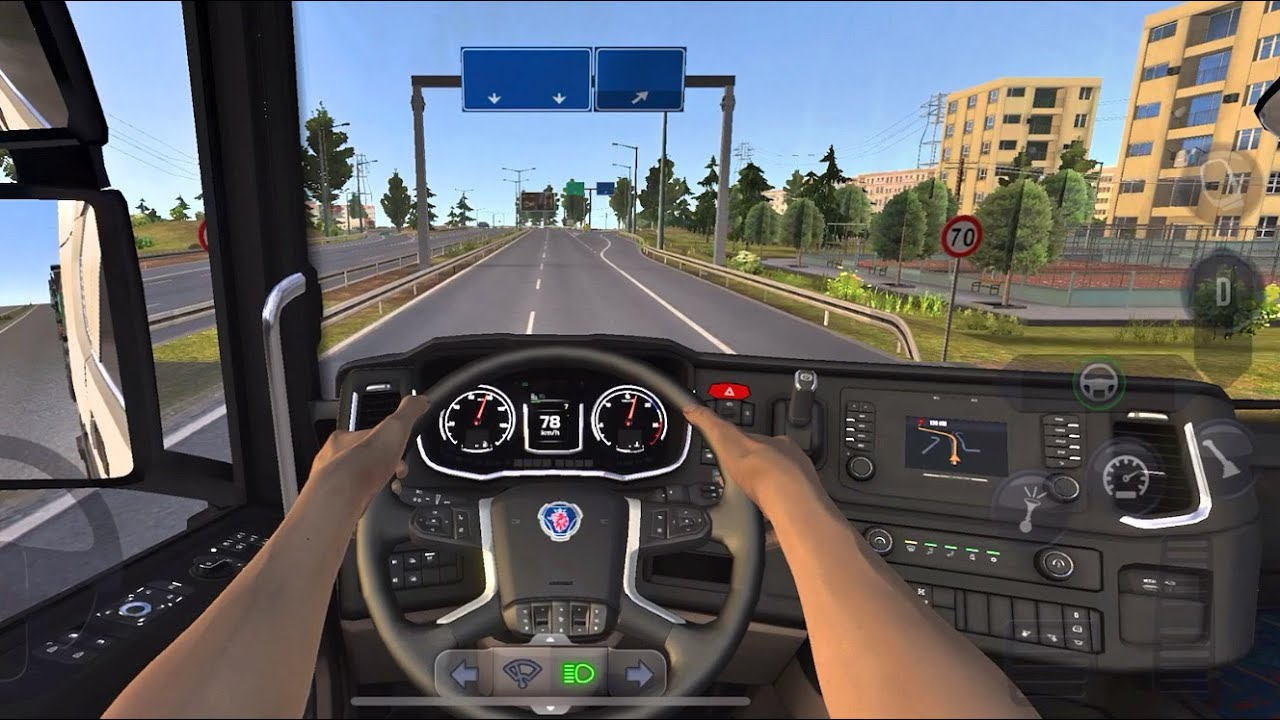
\includegraphics[width=0.6\textwidth]{playwright_figures/sim_arch.png}
    \end{columns}
    \note[item]{Вводный слайд. Симуляторы экономят деньги и время. Важно понимать, что симулятор состоит из графики, физики и моста к ROS.}
\end{frame}

\begin{frame}[t]{Physics Engines: The Math Behind Simulation}
    \begin{columns}
        \column{0.6\textwidth}
        \begin{itemize}
            \item \textbf{Simulator vs. Engine:} A simulator provides the UI and rendering. The physics engine solves the math.
            \item \textbf{Common Physics Engines:}
            \begin{itemize}
                \item \textbf{ODE:} Classic, used in older Gazebo.
                \item \textbf{Bullet / PyBullet:} Popular in RL and robotics.
                \item \textbf{DART:} Focuses on articulated dynamics.
                \item \textbf{MuJoCo Engine:} Optimized for contact dynamics.
            \end{itemize}
        \end{itemize}
        \column{0.4\textwidth}
        \centering
        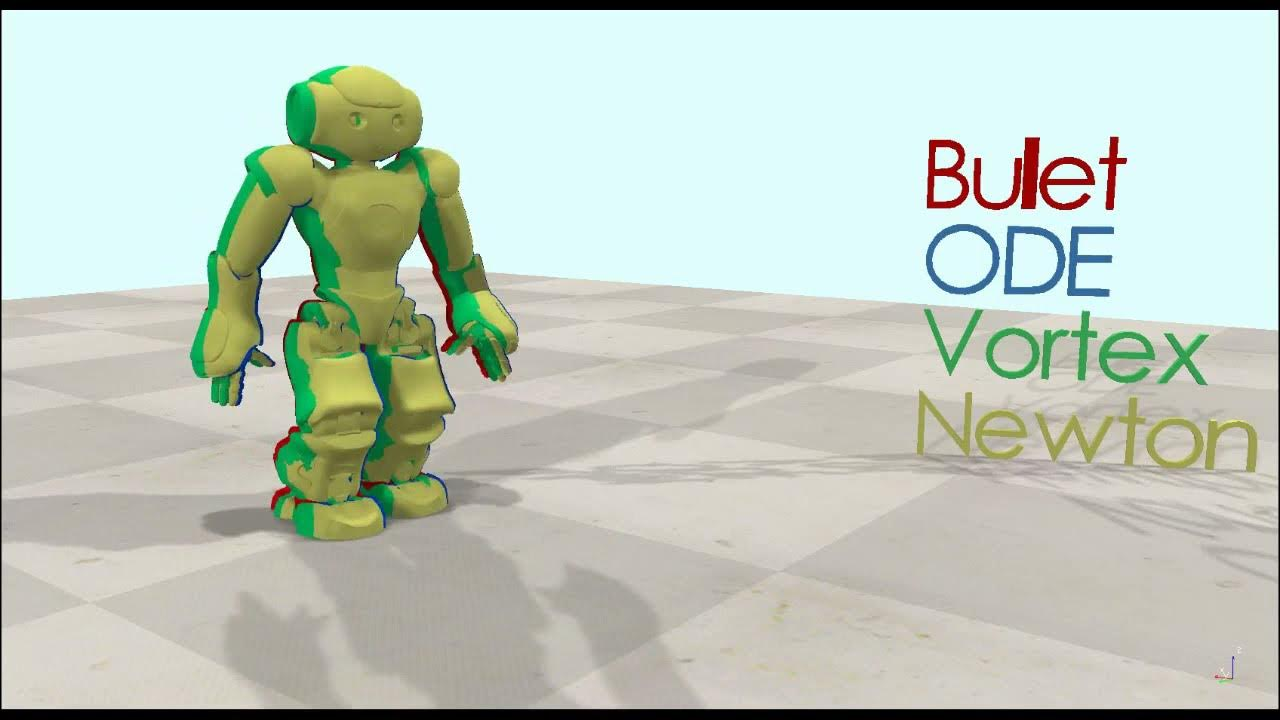
\includegraphics[width=0.8\textwidth]{playwright_figures/physics_engines.png}
    \end{columns}
    \note[item]{Важно понимать разницу: симулятор — это оболочка, а движок — это математика внутри. От движка зависит, провалится ли робот сквозь пол.}
\end{frame}

\begin{frame}[t]{Gazebo: The ROS Standard}
    \begin{columns}
        \column{0.5\textwidth}
        \textbf{Gazebo Classic (ROS 1 / early ROS 2)}
        \begin{itemize}
            \item Monolithic architecture.
            \item Uses ODE by default.
            \item Simple rendering (sufficient for navigation).
        \end{itemize}
        \vspace{0.1cm}
        \centering
        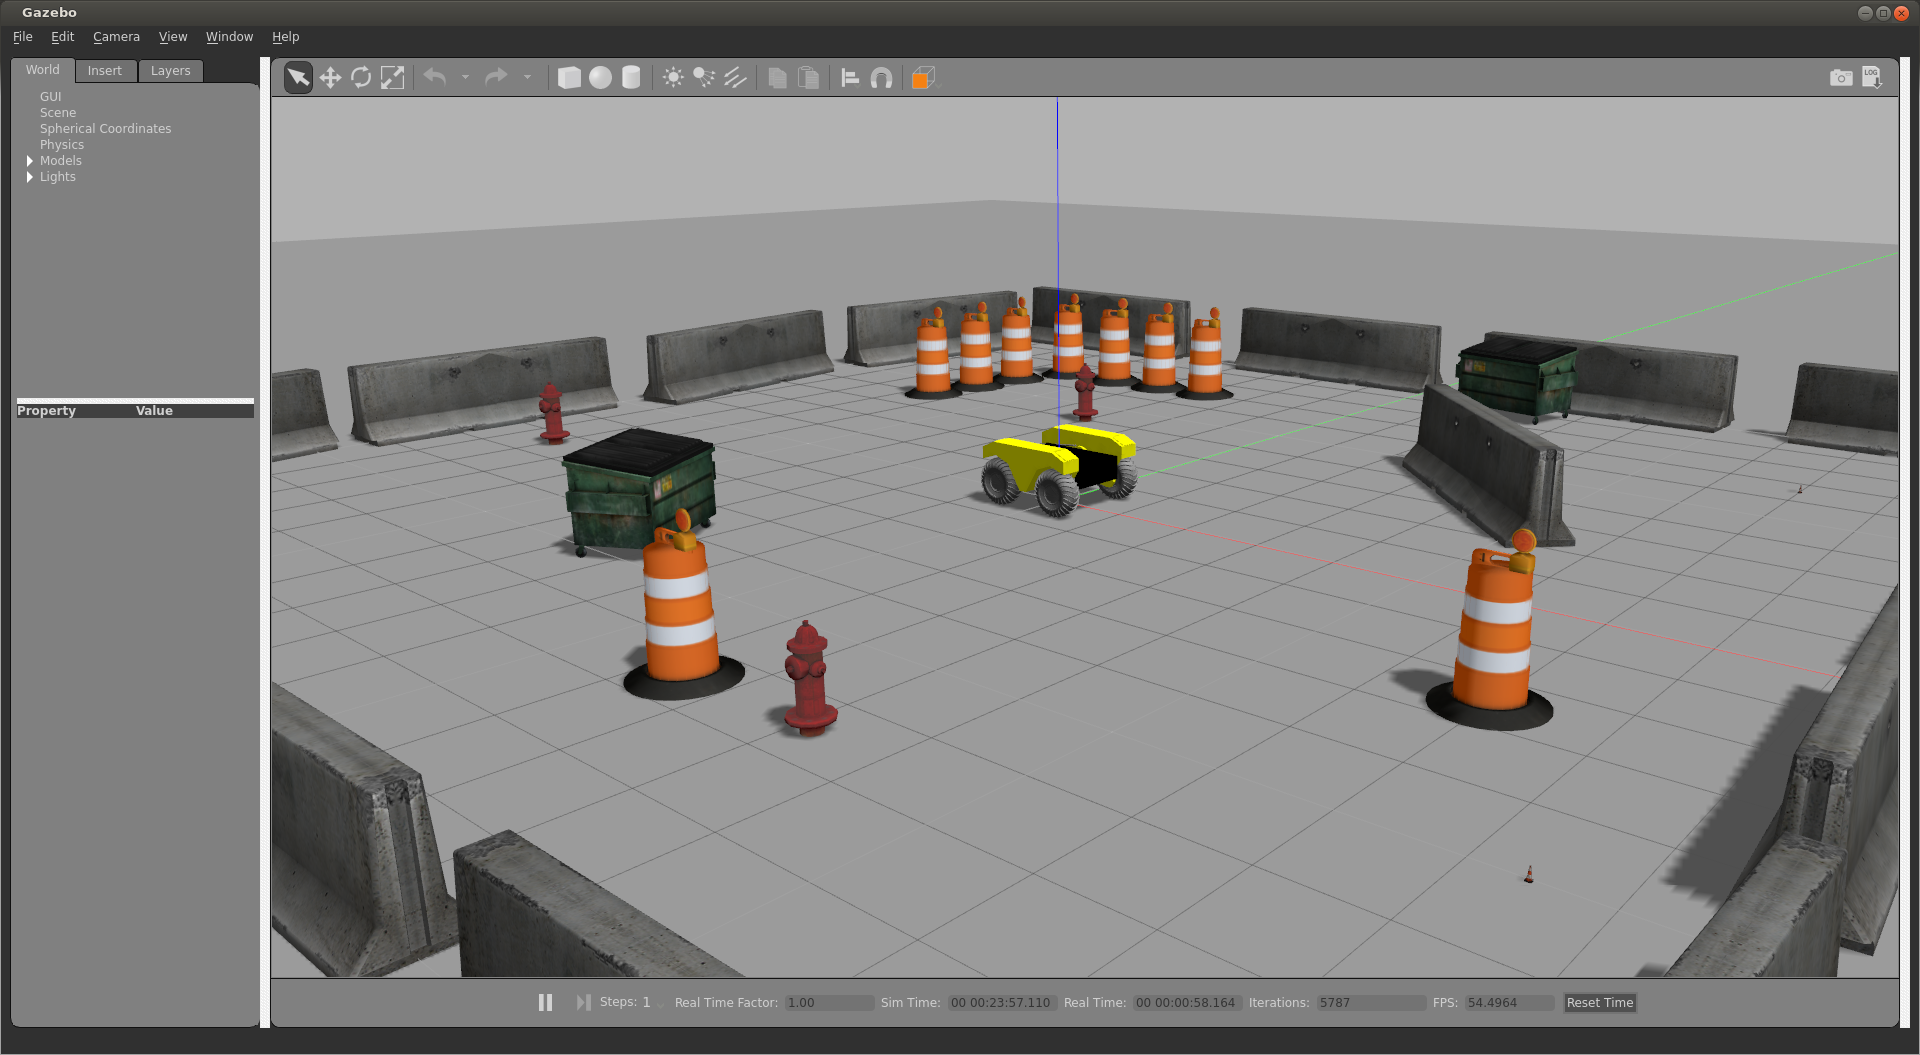
\includegraphics[width=0.8\textwidth]{playwright_figures/gazebo.png}
        
        \column{0.5\textwidth}
        \textbf{Modern Gazebo (Ignition / Harmonic)}
        \begin{itemize}
            \item Modular architecture (plugins).
            \item Supports multiple physics engines (DART, Bullet).
            \item Improved rendering (PBR).
        \end{itemize}
        \vspace{0.1cm}
        \centering
        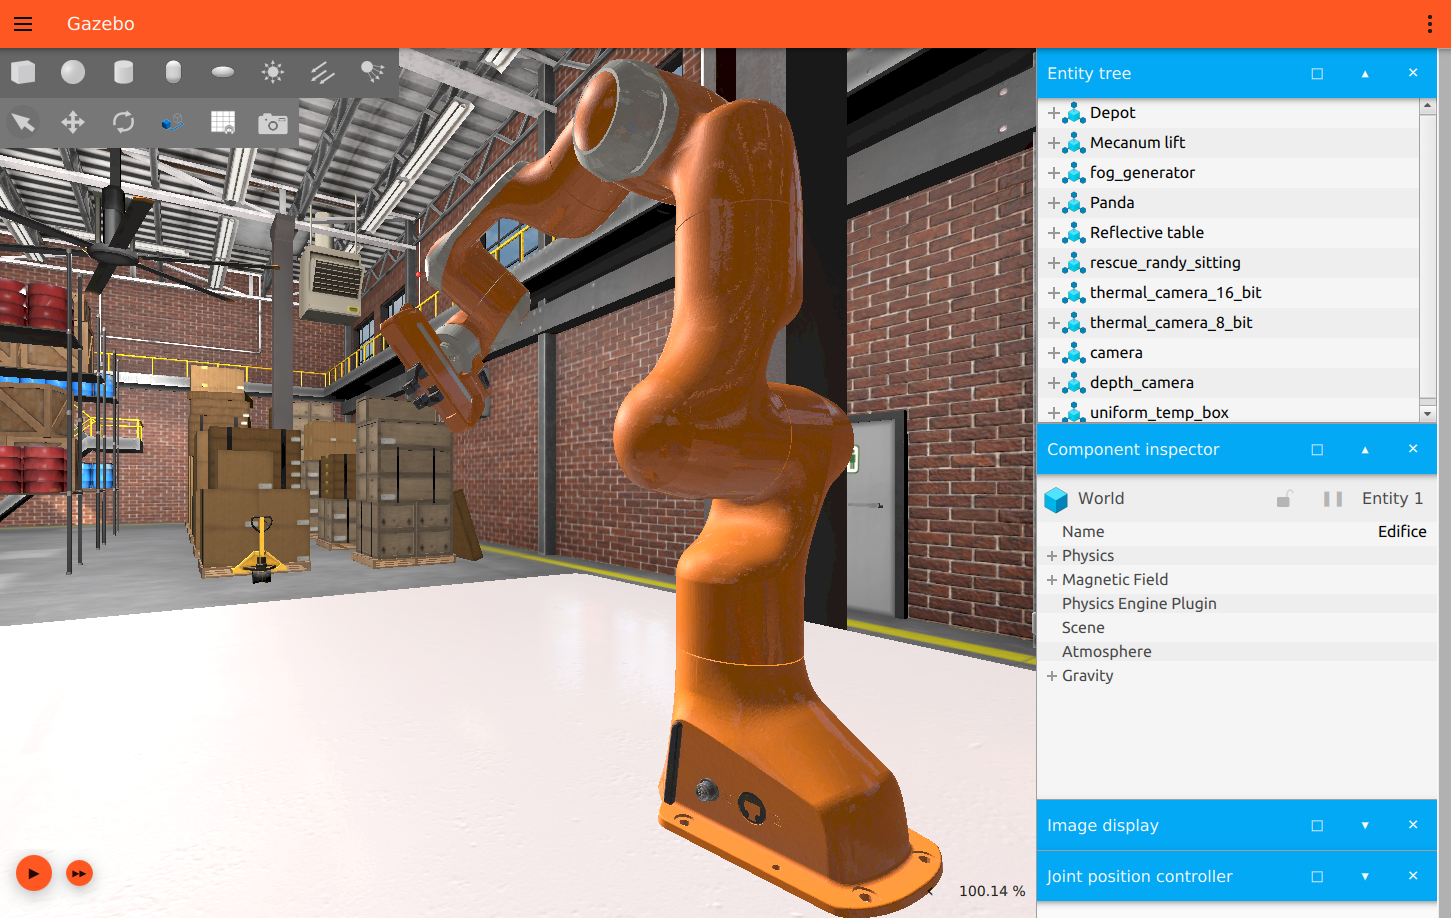
\includegraphics[width=0.8\textwidth]{playwright_figures/gazebo_ignition.png}
    \end{columns}
    \note[item]{Gazebo — стандарт де-факто. Classic уходит в прошлое, Modern (Ignition) — будущее. Рендер простой, но для лидаров и навигации этого достаточно.}
\end{frame}

\begin{frame}[t]{CoppeliaSim (formerly V-REP)}
    \begin{columns}
        \column{0.5\textwidth}
        \begin{itemize}
            \item \textbf{Flexibility:} Highly scriptable using Lua, Python, C++, or MATLAB.
            \item \textbf{Assets:} Comes with a massive library of pre-built robots, sensors, and environments.
            \item \textbf{Engines:} Supports Bullet, ODE, Newton, and Vortex.
            \item \textbf{Use Case:} Rapid prototyping and factory automation simulation.
        \end{itemize}
        \column{0.5\textwidth}
        \centering
        \vfill
        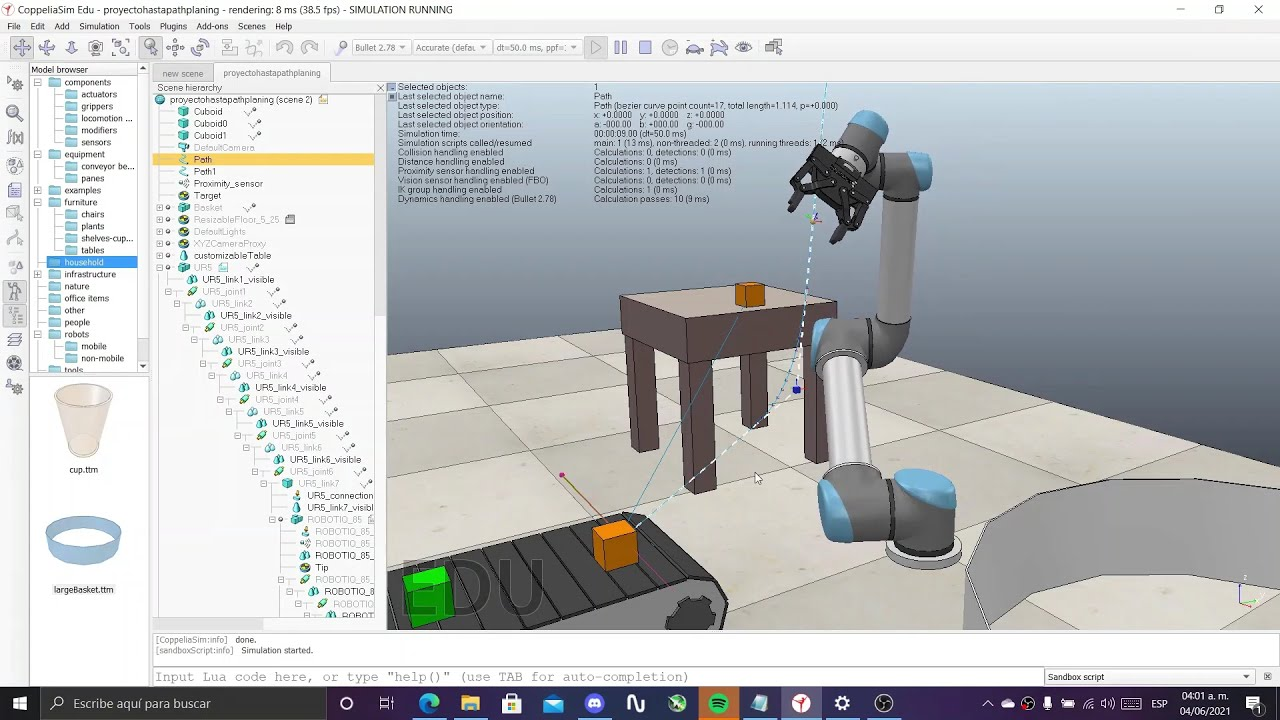
\includegraphics[width=\textwidth]{playwright_figures/coppeliasim.png}
        \vfill
    \end{columns}
    \note[item]{CoppeliaSim (V-REP) любят за огромную библиотеку готовых роботов и возможность писать скрипты на Lua прямо внутри сцены.}
\end{frame}

\begin{frame}[t]{Isaac Sim: Photorealism and GPU Power}
    \begin{columns}
        \column{0.5\textwidth}
        \begin{itemize}
            \item \textbf{Engine:} NVIDIA PhysX (GPU accelerated).
            \item \textbf{Photorealism:} Ray tracing and advanced lighting.
            \item \textbf{Why is photorealism important?}
            \begin{itemize}
                \item Generating synthetic data for Computer Vision.
                \item Sim2Real transfer for Reinforcement Learning (RL).
                \item If the sim looks real, the AI performs better in reality.
            \end{itemize}
        \end{itemize}
        \column{0.5\textwidth}
        \centering
        \vfill
        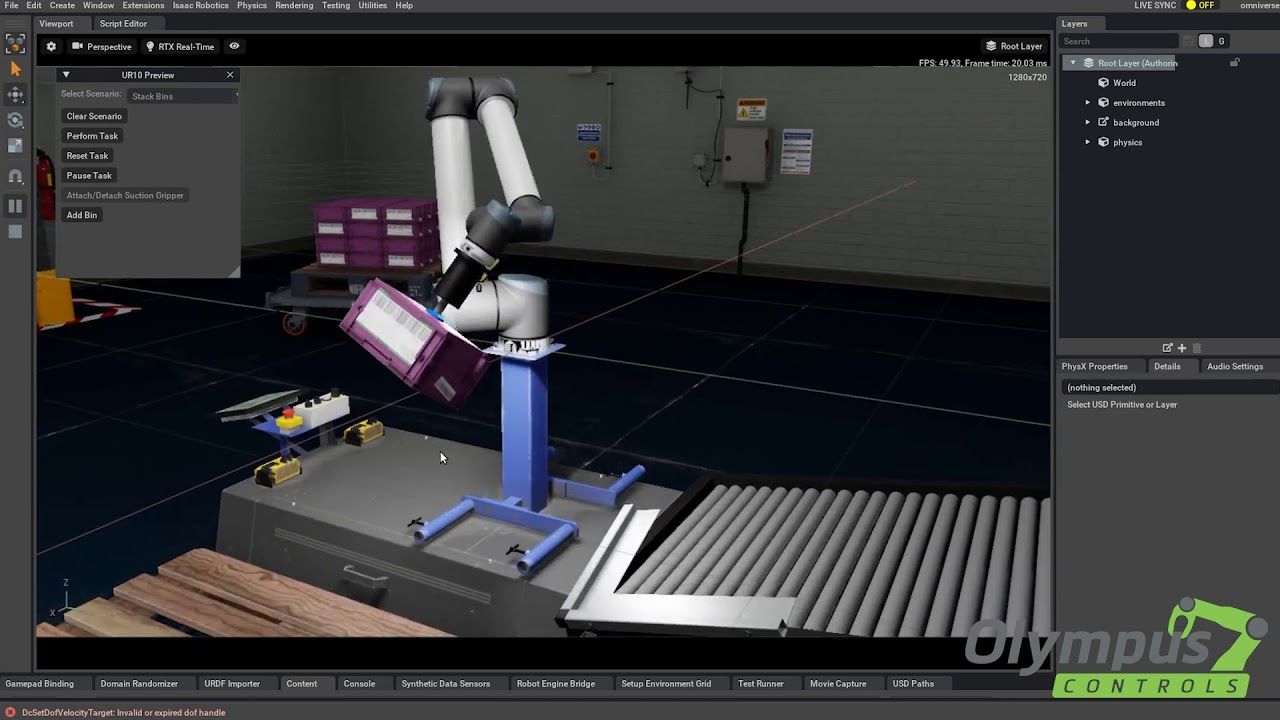
\includegraphics[width=\textwidth]{playwright_figures/isaac_sim.png}
        \vfill
    \end{columns}
    \note[item]{Isaac Sim от NVIDIA. Главная фишка — фотореализм. Это критически важно для обучения нейросетей (CV, RL), чтобы они не пугались реального мира после симуляции.}
\end{frame}

\begin{frame}[t]{MuJoCo and ManiSkill: RL and Manipulation}
    \begin{columns}
        \column{0.5\textwidth}
        \textbf{MuJoCo}
        \begin{itemize}
            \item Exceptional at handling complex contact dynamics.
            \item Extremely fast CPU performance.
            \item Standard for continuous control RL tasks.
        \end{itemize}
        \vspace{0.05cm}
        \textbf{ManiSkill}
        \begin{itemize}
            \item Built on SAPIEN (Vulkan-based).
            \item Specialized for robotic manipulation tasks.
            \item Massive GPU parallelization for RL
        \end{itemize}
        \column{0.5\textwidth}
        \centering
        \vfill
        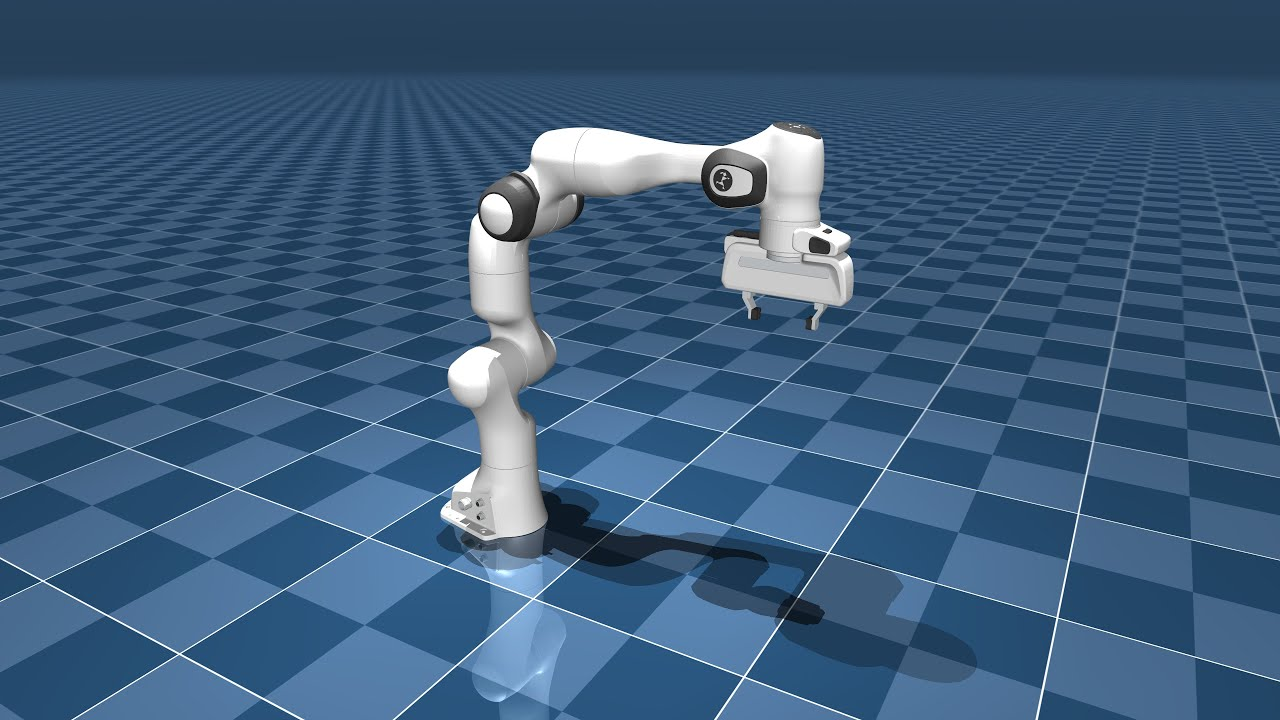
\includegraphics[width=0.55\textwidth]{playwright_figures/mujoco.jpg}
        \vfill
        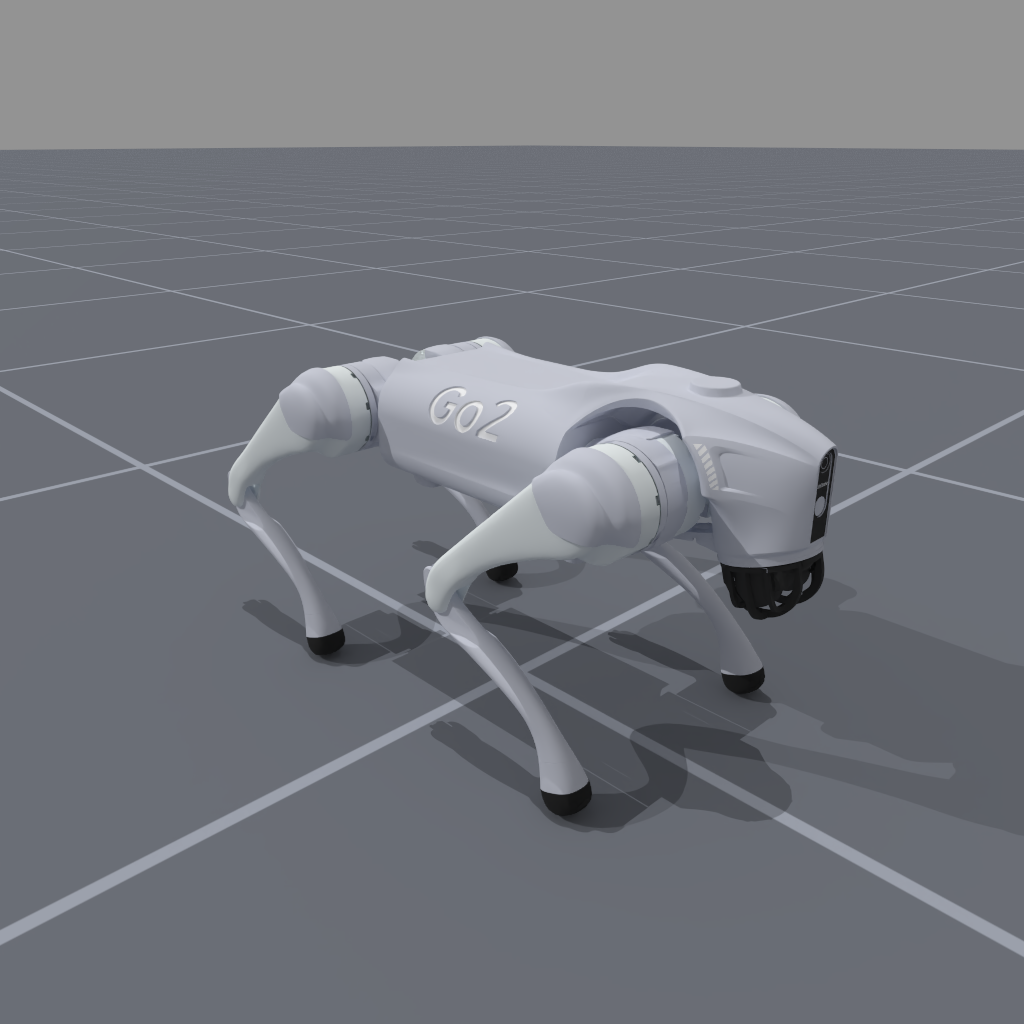
\includegraphics[width=0.55\textwidth]{playwright_figures/maniskill.png}
        \vfill
    \end{columns}
    \note[item]{MuJoCo — король контактов и RL. ManiSkill позволяет запускать тысячи симуляций параллельно на одной видеокарте, ускоряя обучение в сотни раз.}
\end{frame}

\begin{frame}[t]{Chapter 1 References}
    \begin{itemize}
        \item \href{https://gazebosim.org}{Gazebo Official Website}
        \item \href{https://mujoco.org}{MuJoCo Physics Engine}
        \item \href{https://maniskill.ai}{ManiSkill Project Page}
        \item \href{https://developer.nvidia.com/isaac-sim}{NVIDIA Isaac Sim}
        \item \href{https://www.coppeliarobotics.com/}{CoppeliaSim Official Website}
    \end{itemize}
\end{frame}

% --- CHAPTER 2: URDF ---
\section{Robot Description (URDF)}

\begin{frame}[t]{Unified Robot Description Format (URDF)}
    \begin{itemize}
        \item \textbf{Definition:} XML-based format describing the physical structure of a robot in ROS.
        \item \textbf{Purpose:} Centralizes kinematics, visual appearance, and collision properties.
        \item \textbf{Core Components:}
        \begin{itemize}
            \item \textbf{Links:} Rigid bodies (e.g., chassis, wheels) with inertia, visual, and collision data.
            \item \textbf{Joints:} Connections between links (revolute, continuous, fixed, etc.).
        \end{itemize}
        \item \textbf{Xacro:} XML Macros to make URDF modular, reusable, and parameterized.
    \end{itemize}
    \note[item]{URDF — это XML-паспорт робота. Он описывает кости (links) и суставы (joints), чтобы все узлы ROS знали размеры и возможности робота. Xacro позволяет не писать один и тот же код 10 раз.}
\end{frame}

\begin{frame}[fragile,t]{URDF Code Example}
    \begin{columns}[T]
        \column{0.55\textwidth}
        \vspace*{-0.5cm}
\begin{lstlisting}[language=XML]
<robot name="my_robot">
  <link name="gripper_pole">
    <visual>
      <geometry><cylinder length="0.2" radius="0.01"/>
      </geometry>
      <origin rpy="0 1.57075 0 " xyz="0.1 0 0"/>
    </visual>
  </link>

  <joint name="left_gripper_joint" type="fixed">
    <origin rpy="0 0 0" xyz="0.2 0.01 0"/>
    <parent link="gripper_pole"/>
    <child link="left_gripper"/>
  </joint>

  <link name="left_gripper">
    <visual><origin rpy="0.0 0 0" xyz="0 0 0"/>
      <geometry>
        <mesh filename="package://urdf_tutorial/meshes/l_finger.dae"/>
      </geometry>
    </visual></link>
</robot>
\end{lstlisting}
        \column{0.45\textwidth}
        \centering
        \vfill
        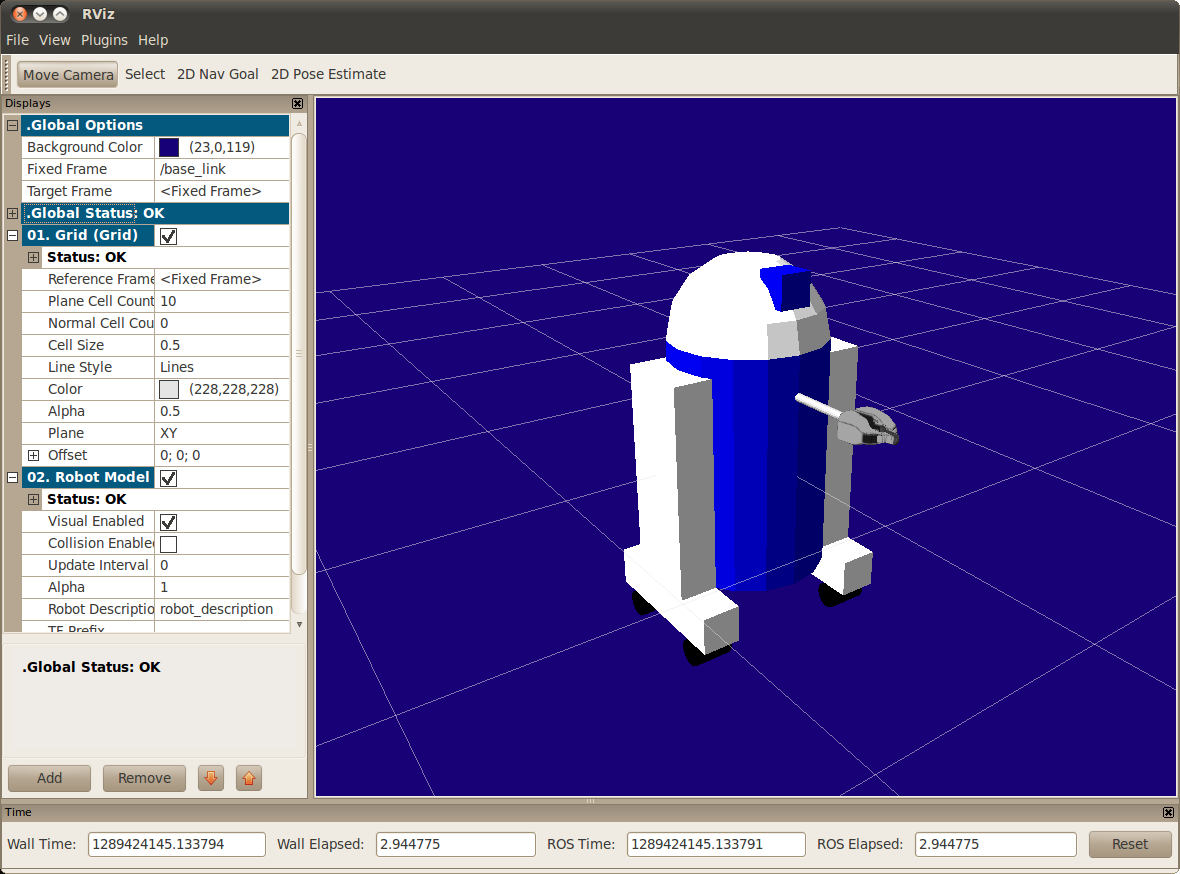
\includegraphics[width=\textwidth]{playwright_figures/rviz_urdf.png}
        \vfill
    \end{columns}
    \note[item]{Пример простого URDF: база и камера, соединенные жестким суставом. Справа должен быть скриншот того, как это выглядит в RViz.}
\end{frame}

\begin{frame}[t]{Chapter 2 References}
    \begin{itemize}
        \item \href{https://docs.ros.org/en/humble/Tutorials/Intermediate/URDF/URDF-Main.html}{ROS 2 URDF Tutorials}
        \item \href{http://sdformat.org}{SDF Specification}
        \item \href{https://mujoco.readthedocs.io/en/stable/modeling.html}{MuJoCo MJCF Modeling Guide}
    \end{itemize}
\end{frame}

% --- CHAPTER 3: TRANSFORM SYSTEM (TF) ---
\section{Transform System (TF)}

\begin{frame}[t]{The Role of Coordinate Frames (TF2)}
    \begin{itemize}
        \item \textbf{Concept:} Robots operate with multiple coordinate systems (frames). TF tracks these frames over time.
        \item \textbf{Structure:} A tree hierarchy where every frame has exactly one parent (no closed loops).
        \item \textbf{Types of Transforms:}
        \begin{itemize}
            \item \textbf{Static:} Constant over time (e.g., sensor bolted to chassis). Published to \texttt{/tf\_static}.
            \item \textbf{Dynamic:} Continuously updated (e.g., moving wheels, robot in map). Published to \texttt{/tf}.
        \end{itemize}
        \item \textbf{robot\_state\_publisher:} Node that reads URDF and joint states to publish the internal TF tree.
    \end{itemize}
    \note[item]{Система TF отвечает на вопрос «где находится предмет Х относительно руки робота?». Она строит дерево систем координат, где все связано через родительские и дочерние связи.}
\end{frame}

\begin{frame}[t]{TF Tree Example}
    \begin{figure}[H]
        \centering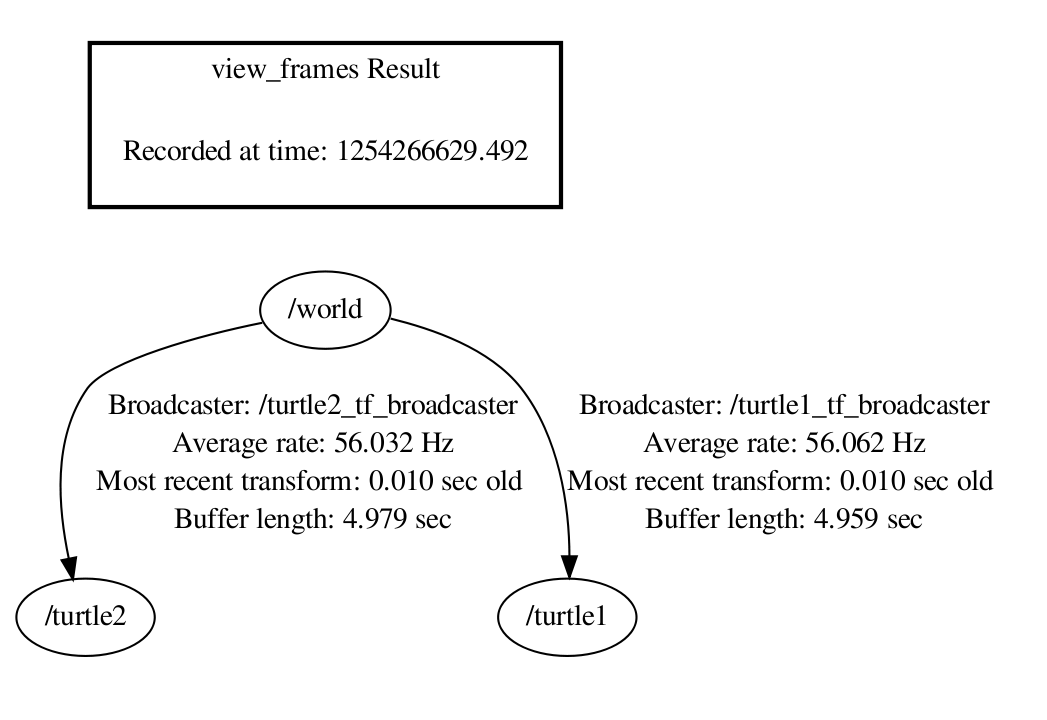
\includegraphics[height=6cm,width=1\textwidth,keepaspectratio]{playwright_figures/view_frames_2.png}
        \label{fig:tf_tree_example}
    \end{figure}
\end{frame}

\begin{frame}[fragile,t]{TF and Sensor Data (std\_msgs/Header)}
    \begin{itemize}
        \item Sensor data (e.g., \texttt{LaserScan}, \texttt{Image}) must be linked to the TF tree.
        \item This is done via the \texttt{std\_msgs/Header} message type.
        \item \textbf{frame\_id:} Specifies which TF frame the data belongs to.
        \item \textbf{stamp:} The exact time the data was captured (crucial for dynamic transforms).
    \end{itemize}
\begin{lstlisting}[language=bash]
# Example of a Header in a ROS 2 message
header:
  stamp:
    sec: 1623456789
    nanosec: 123456789
  frame_id: 'lidar_link'
\end{lstlisting}
    \note[item]{Данные с лидара бесполезны, если мы не знаем, где он находится. Поле frame\_id в заголовке сообщения связывает данные с конкретным узлом в дереве TF.}
\end{frame}

\begin{frame}[fragile,t]{TF CLI Commands}
    \begin{itemize}
        \item \textbf{Publish a static transform manually:}
\begin{lstlisting}[language=bash]
ros2 run tf2_ros static_transform_publisher x y z yaw pitch roll frame_id child_frame_id
ros2 run tf2_ros static_transform_publisher 0.1 0 0.2 0 0 0 base_link camera_link
\end{lstlisting}
        \item \textbf{View the current TF tree (generates a PDF):}
\begin{lstlisting}[language=bash]
ros2 run tf2_tools view_frames
\end{lstlisting}
        \item \textbf{Print the transform between two frames:}
\begin{lstlisting}[language=bash]
ros2 run tf2_ros tf2_echo map base_link
\end{lstlisting}
    \end{itemize}
    \note[item]{Практические команды. static\_transform\_publisher часто используется для быстрой проверки или временных костылей. view\_frames — главный инструмент дебага.}
\end{frame}

\begin{frame}[t]{Chapter 3 References}
    \begin{itemize}
        \item \href{https://docs.ros.org/en/humble/Concepts/Intermediate/About-Tf2.html}{Introduction to tf2}
        \item \href{https://www.ros.org/reps/rep-0105.html}{REP-105: Coordinate Frames standard}
    \end{itemize}
\end{frame}

% --- CHAPTER 4: NAMESPACES ---
\section{Namespaces in ROS 2}

\begin{frame}[t]{Namespace Isolation}
    \begin{itemize}
        \item \textbf{Problem:} Multiple robots in one network will publish to the same topics (e.g., \texttt{/cmd\_vel}), causing conflicts.
        \item \textbf{Solution:} Namespaces group nodes, topics, and services under a specific prefix.
        \item \textbf{Result:} \texttt{/robot1/cmd\_vel} is completely isolated from \texttt{/robot2/cmd\_vel}.
    \end{itemize}
    \vspace{0.1cm}
    \centering
    \begin{tikzpicture}[
        scale=0.75, transform shape,
        node distance=0.6cm and 1.5cm,
        topic/.style={ellipse, draw=green!60, fill=green!5, thick, minimum size=5mm},
        node_ros/.style={rectangle, draw=red!60, fill=red!5, thick, minimum size=5mm, rounded corners},
        arrow/.style={->, thick, >=stealth}
    ]
    \node[node_ros] (teleop1) {Teleop};
    \node[topic] (cmd1) [right=of teleop1] {/robot1/cmd\_vel};
    \node[node_ros] (base1) [right=of cmd1] {Base Controller};
    
    \node[node_ros] (teleop2) [below=of teleop1] {Teleop};
    \node[topic] (cmd2) [right=of teleop2] {/robot2/cmd\_vel};
    \node[node_ros] (base2) [right=of cmd2] {Base Controller};

    \draw[arrow] (teleop1) -- (cmd1);
    \draw[arrow] (cmd1) -- (base1);
    \draw[arrow] (teleop2) -- (cmd2);
    \draw[arrow] (cmd2) -- (base2);
    \end{tikzpicture}
    \note[item]{Неймспейсы — это как папки на диске. Они позволяют запускать несколько узлов с одинаковыми именами, не боясь, что топики перемешаются. Критично для мультиагентных систем.}
\end{frame}

\begin{frame}[fragile,t]{Using Namespaces via CLI}
    \begin{itemize}
        \item You can push a node into a namespace directly from the command line using \texttt{--ros-args -r \_\_ns:=<namespace>}.
    \end{itemize}
\begin{lstlisting}[language=bash]
# Run a talker node in the /robot1 namespace
ros2 run demo_nodes_cpp talker --ros-args -r __ns:=/robot1

# Check the topics
ros2 topic list
# Output will include: /robot1/chatter
\end{lstlisting}
    \begin{itemize}
        \item In launch files, the \texttt{PushRosNamespace} action is used to apply a namespace to an entire group of nodes.
    \end{itemize}
    \note[item]{Пример того, как легко переопределить неймспейс при запуске. В launch-файлах это делается еще проще для целых групп узлов.}
\end{frame}

\begin{frame}[t]{Namespaces and the TF Problem}
    \begin{itemize}
        \item \textbf{The TF Exception:} By default, \texttt{/tf} and \texttt{/tf\_static} are \textbf{global} topics. They are usually NOT namespaced.
        \item \textbf{Why?} The TF tree is designed to be a single, unified graph for the entire system.
        \item \textbf{Namespacing TF:} You \textit{can} push TF into a namespace (e.g., \texttt{/robot1/tf}), but it causes problems:
        \begin{itemize}
            \item Standard tools (like RViz) expect a global \texttt{/tf} topic.
            \item In code, \texttt{tf2\_ros::TransformListener} uses a special mechanism to subscribe to TF. It does not read TF like a normal topic.
            \item If TF is namespaced, you must explicitly remap the listener's topics or configure it to use the specific namespace, which is error-prone.
        \end{itemize}
        \item \textbf{Best Practice:} Keep \texttt{/tf} global, but prefix the \texttt{frame\_id}s (e.g., \texttt{robot1/base\_link}).
    \end{itemize}
    \note[item]{TF — это боль при работе с неймспейсами. Обычно топик /tf один на всех, а разделение идет внутри самих сообщений через префиксы frame\_id. Если разделить сам топик, придется переписывать код листенеров, так как они читают TF через специальный механизм.}
\end{frame}

\begin{frame}[t]{Chapter 4 References}
    \begin{itemize}
        \item \href{https://docs.ros.org/en/humble/Concepts/Basic/About-Nodes.html\#namespaces}{ROS 2 Nodes and Namespaces}
        \item \href{https://navigation.ros.org/setup_guides/index.html}{Nav2 Multi-Robot Setup Guide}
    \end{itemize}
\end{frame}

% --- CHAPTER 5: DDS AND ZENOH ---
\section{DDS and Zenoh Communication}

\begin{frame}[t]{FastDDS vs. CycloneDDS}
    \begin{columns}
        \column{0.5\textwidth}
        \textbf{FastDDS (eProsima)}
        \begin{itemize}
            \item Default in ROS 2 Foxy/Humble.
            \item \textbf{Pros:} Out-of-the-box Shared Memory (SHM) for zero-copy local transfers. Discovery Server feature solves Wi-Fi issues.
            \item \textbf{Cons:} Default multicast discovery floods Wi-Fi networks. Complex XML configuration.
        \end{itemize}
        \column{0.5\textwidth}
        \textbf{CycloneDDS (Eclipse)}
        \begin{itemize}
            \item Default in ROS 2 Galactic.
            \item \textbf{Pros:} Excellent "out-of-the-box" stability on lossy networks (Wi-Fi). Simple configuration. Lightweight.
            \item \textbf{Cons:} Lacks native zero-copy SHM (requires iceoryx integration). Less performant for massive local payloads.
        \end{itemize}
    \end{columns}
    \vspace{0.1cm}
    \begin{itemize}
        \item \textbf{Verdict:} Use \textbf{CycloneDDS} for stable multi-robot Wi-Fi setups. Use \textbf{FastDDS} for high-performance single-machine systems (cameras/lidars) or complex WANs.
    \end{itemize}
    \note[item]{FastDDS мощный, поддерживает Shared Memory для тяжелых данных, но по умолчанию кладет Wi-Fi мультикастом. CycloneDDS работает "из коробки" и отлично держит Wi-Fi. Для большинства лабораторных задач CycloneDDS предпочтительнее.}
\end{frame}

\begin{frame}[fragile,t]{DDS (Data Distribution Service)}
    \begin{columns}
        \column{0.6\textwidth}
        \begin{itemize}
            \item \textbf{Concept:} Data-centric, peer-to-peer protocol with rich QoS settings.
            \item \textbf{FastDDS:} Default in ROS 2 Humble.
            \item \textbf{CycloneDDS:} Often considered more stable "out of the box".
            \item \textbf{Switching DDS:}
        \end{itemize}
\begin{lstlisting}[language=bash]
# Install CycloneDDS
sudo apt install ros-humble-rmw-cyclonedds-cpp

# Switch implementation
export RMW_IMPLEMENTATION=rmw_cyclonedds_cpp
\end{lstlisting}
        \column{0.4\textwidth}
        \centering
        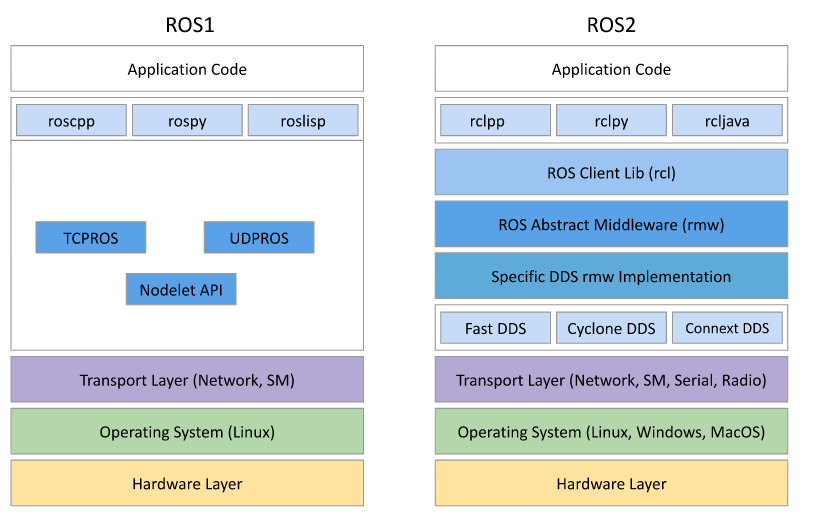
\includegraphics[width=\textwidth]{playwright_figures/dds_diagram.png}
    \end{columns}
    \note[item]{DDS — это стандартный «двигатель» связи в ROS 2. FastDDS стоит по умолчанию, но CycloneDDS часто работает стабильнее без долгой настройки XML-файлов.}
\end{frame}

\begin{frame}[t]{Zenoh: Bridging the WAN Gap}
    \begin{itemize}
        \item \textbf{The Problem:} DDS relies on multicast for discovery, which fails over Wi-Fi, VPNs, or Wide Area Networks (WAN).
        \item \textbf{Zenoh:} A "Zero Overhead" protocol designed for efficiency and scale.
        \item \textbf{zenoh-plugin-dds:} Acts as a bridge, transparently routing DDS traffic across a Zenoh network (e.g., Robot to Cloud).
    \end{itemize}
    \vspace{0.05cm}
    \centering
    \begin{tikzpicture}[
        scale=0.65, transform shape,
        node distance=0.8cm and 0.5cm,
        dds/.style={ellipse, draw=orange!60, fill=orange!5, thick, minimum size=5mm},
        zenoh/.style={rectangle, draw=purple!60, fill=purple!5, thick, minimum size=5mm, rounded corners},
        arrow/.style={<->, thick, >=stealth}
    ]
    \node[dds] (ros1) {ROS 2 (Robot)};
    \node[zenoh] (bridge1) [right=of ros1] {Zenoh Bridge};
    \node[ellipse, draw=gray!60, fill=gray!5, thick, minimum width=2cm, minimum height=1cm] (internet) [right=of bridge1] {Internet / WAN};
    \node[zenoh] (bridge2) [right=of internet] {Zenoh Bridge};
    \node[dds] (ros2) [right=of bridge2] {ROS 2 (Cloud)};

    \draw[arrow] (ros1) -- node[above] {DDS} (bridge1);
    \draw[arrow] (bridge1) -- node[above] {Zenoh} (internet);
    \draw[arrow] (internet) -- node[above] {Zenoh} (bridge2);
    \draw[arrow] (bridge2) -- node[above] {DDS} (ros2);
    \end{tikzpicture}
    \note[item]{Zenoh решает главную боль DDS — работу через интернет. Мост Zenoh берет локальный DDS-трафик робота и прокидывает его на сервер без мультикаста.}
\end{frame}

\begin{frame}[t]{Chapter 5 References}
    \begin{itemize}
        \item \href{https://zenoh.io}{Zenoh Official Website}
        \item \href{https://github.com/eclipse-zenoh/zenoh-plugin-dds}{Zenoh DDS Plugin GitHub}
        \item \href{https://www.omg.org/spec/DDS/}{OMG DDS Specification}
    \end{itemize}
\end{frame}

% --- CHAPTER 6: TESTING ---
\section{Testing in ROS 2}

\begin{frame}[t]{Why Test in Robotics?}
        \begin{itemize}
            \item \textbf{Safety:} Prevent regressions that could damage hardware.
            \item \textbf{CI/CD Integration:} Automatically validate code on every commit.
            \item \textbf{Edge Cases:} Safely test dangerous scenarios in simulation.
            \item \textbf{Benchmarking:} Quantitatively measure performance metrics.
        \end{itemize}
    \note[item]{Тесты в симуляции — это гарантия безопасности. Сначала проверяем всё в «цифре», считаем метрики успеха, и только потом идем к реальному роботу.}
\end{frame}

\begin{frame}[fragile,t]{Levels of Testing in ROS 2}
    \begin{itemize}
        \item \textbf{Unit Tests (GTest / Pytest):} Test individual functions or classes in isolation.
        \item \textbf{Integration Tests (\texttt{launch\_testing}):} Test the interaction between multiple ROS nodes (e.g., does Node A correctly process messages from Node B?).
        \item \textbf{System / SITL Tests:} "Simulation-in-the-loop". Run the entire software stack against a physics simulator to validate complex behaviors.
    \end{itemize}
\begin{lstlisting}[language=bash]
# Build tests
colcon build --packages-select my_package --cmake-args -DBUILD_TESTING=ON

# Run tests
colcon test --packages-select my_package

# View results
colcon test-result --all
\end{lstlisting}
    \note[item]{В ROS 2 есть три уровня тестов: проверка отдельных функций, проверка связей между узлами и полная проверка поведения робота в симуляторе. Команды colcon позволяют автоматизировать этот процесс.}
\end{frame}

\begin{frame}[t]{Chapter 6 References}
    \begin{itemize}
        \item \href{https://docs.ros.org/en/humble/Tutorials/Intermediate/Testing/Testing-Main.html}{ROS 2 Testing Guide}
        \item \href{https://colcon.readthedocs.io/en/released/user/test.html}{Colcon Testing Documentation}
    \end{itemize}
\end{frame}

\fbckg{fibeamer/figs/last_page.png}
\frame[plain]{}

\end{document}
